\chapter{General Configuration Management in MADTrack}\label{cap:Milestone3}

One of the main milestones presented within the previous chapter is milestone 3 (codename \emph{G}), which is focused on the development of features related to General
Configuration Management. The main purpose of developing these features as a separate module is to provide an extensible basis for possible future developments of features
unrelated to versioning datasets and models, and more related to basic configuration management mechanisms. In this chapter, a brief introduction to what needs to be developed
will be made, as well as an analysis of the requirements that will need to be developed for this milestone, which will result in a diagnosis of the most suitable architecture
and application type for this module.

\section{Introduction}

The partial objectives of the project are related to configuration management applied to datasets and models, but the development of such a system will depend on more generic
configuration management mechanisms. In fact, it is shown in the project's roadmap (\emph{figure \ref{fig:roadmap}}) that the development of the general configuration management
features is crucial for initiating the development in the rest of the milestones' prototypes. Hence, the development of this module will be focused on creating mechanisms that interact
synergically with the rest of the components, mainly in the cases where commits to remote or local repositories are required.

\section{Requirements analysis for milestone 3}

The main purpose of analysis is to define the most suitable way to proceed with the development of the prototypes. In this case, the functionalities provided by Git are the 
are the ones most suitable to use in the context of development. This Prototype interacts with all those prototypes that require integrating changes to the system, such as 
tracking and committing changes within a dataset or a model.

\subsection{Requirements involved}

The requirements involved within this milestone have already been listed within \emph{table \ref{tab:requirementsMilestone3}}. These requirements all belong to prototype \emph{G1}, which
is the first one to be completed, and the only one belonging to this milestone.

Additionally, prototypes within milestone 3 require the satisfaction of the non-functional requirements listed within \emph{table \ref{tab:nonFunctionalRequirements}}.

\subsection{Integration with the rest of the system}

Prototype G1 is the prototype which constitutes the core dependency for the most prototypes to be developed within the other two milestones. The dependent prototypes are \emph{D2}, which
needs a mechanism for committing changes made to DVC's files, and \emph{M2}, which would potentially need a mechanism for committing metadata stored about training configurations.

\begin{figure}[H]
    \centering
    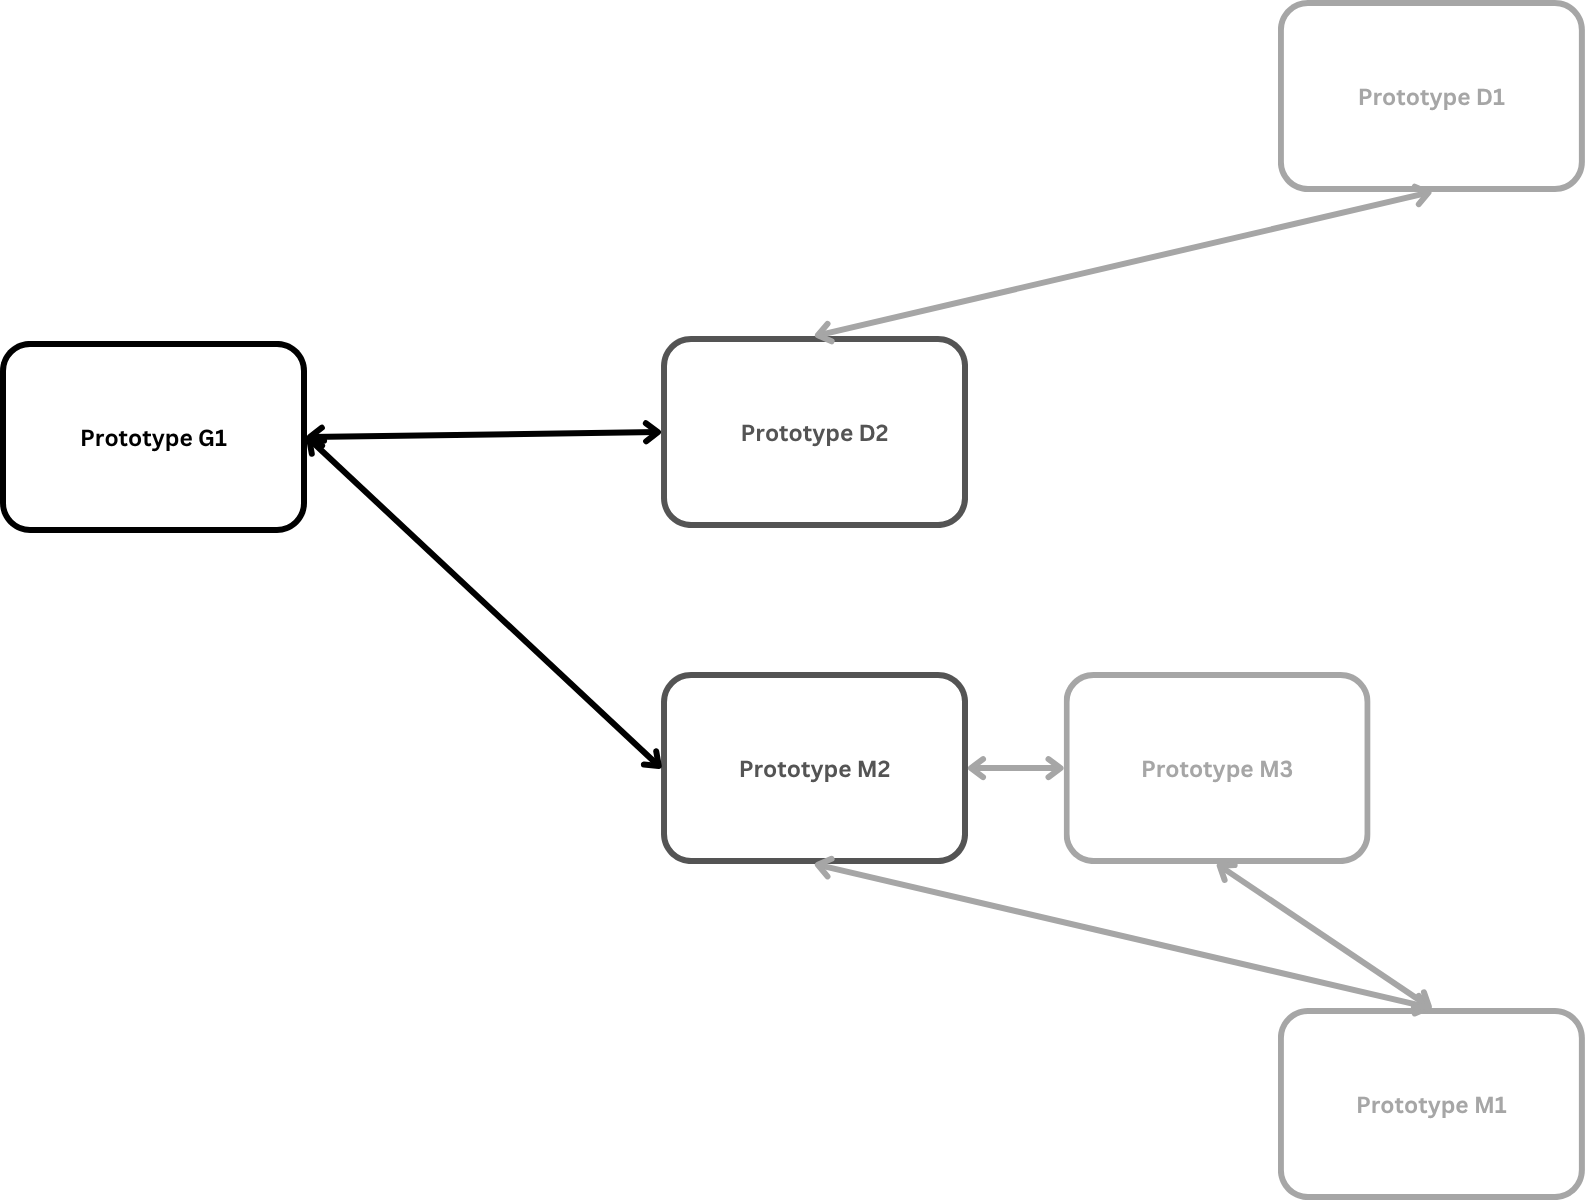
\includegraphics[width=0.7\textwidth]{figs/G-dependencies.png}
    \caption{Dependencies between prototypes of milestone 3 and the rest of the target system, shown by an interaction diagram.}
\end{figure}

\subsection{Architecture analysis}

The nature of the requirements of the milestone describes that multiple aspects shall be handled: The user may want to push their changes to either a local or remote repository. 
And the way to commit changes differs from whether the committed item is a dataset (The information of the DVC tracking file must be committed) or an \acrshort{AI} model (whole model folders can be committed from a repository within
the remote tracking server). Additionally, as versions would be defined by the commit name, a functionality to retrieve the name of the active commit could be useful.

Considering these needs and the aforementioned requirements, the conclusion reached was that the most suitable architecture for the modules of milestone 3 would mainly consist of
a monolithic application, with the possibility for it to connect momentarily to a remote repository server to push changes.

\subsection{Application type analysis}

Due to the reasons described in the previous subsection, the best option for the development of prototypes of this milestone shall be a wrapper library that encapsulates Git
operations. A library that allows to commit to local or remote repository independently of the item to be committed, facilitating thus its integration with toolkits that enable the 
tracking of datasets and models.

\subsection{Toolkit analysis}

Any API or library handling basic Git committing operations will be helpful for the development of the prototypes. Details on the final toolkit used are described in the coming subsections.

\section{Prototype design and development}

Within the coming sections, details for the design, implementation and testing phases of the development of this milestone's prototypes are shown in a sequential order. Since this milestone
is composed of a single prototype, its development will be described in the following subsection.

\subsection{Prototype \emph{G1}}

Prototype G1 is the only prototype of milestone 3, and the core dependency of many other prototypes. It has the aim of bringing basic Git operations to a library accessible to the end users.

\subsubsection{Design for prototype \emph{G1}}

The use case diagram for prototype \emph{G1} is shown in \emph{figure \ref{fig:useCaseG1}}.

\begin{figure}[H]
    \centering
    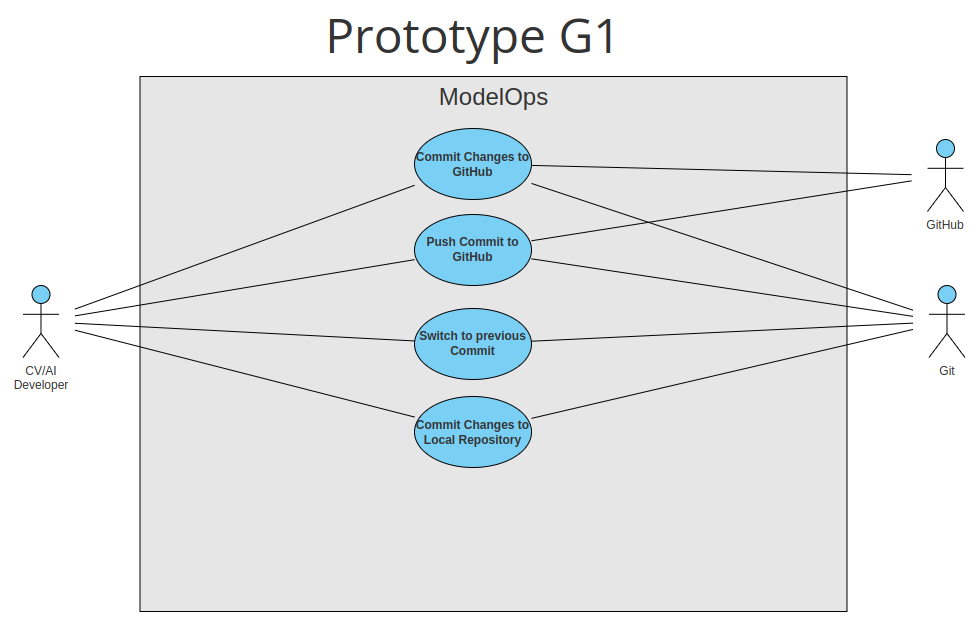
\includegraphics[width=0.7\textwidth]{figs/use-case-G1.png}
    \caption{Use case diagram for prototype \emph{G1}.}
    \label{fig:useCaseG1}
\end{figure}

Taking a look at this diagram, it is clear that there is a crucial component needed to carry out this prototype: a component that handles the Git \emph{commit} and \emph{push} operations, along with
the possible exceptions that this may generate.

\paragraph{Prototype \emph{G1} components}

\begin{itemize}
    \item \textbf{Commit Manager: }a component that will contain the functions for managing both local and remote repositories, as well as operations for changing the active commit (\emph{checkout}).
    
    \item \textbf{Commit Exceptions: }A package that includes some special exceptions that can be raised by the Commit Manager.
\end{itemize}


\paragraph{Design output}\mbox{}\\

The output design class diagram for prototype \emph{G1} is shown in \emph{figure \ref{fig:G1classDiagram}}.

\subsubsection{Implementation for prototype \emph{G1}}

This section addresses questions about the programming language used, the libraries imported, and a high-level description of the implementation of the components' methods.

\paragraph{Libraries used} \mbox{}\\

The libraries used for the implementation of this prototype are:

\begin{itemize}

    \item \textbf{\emph{GitPython}: }the selected toolkit to handle \emph{commit}, \emph{push} and \emph{checkout} operations.
    \item \textbf{\emph{Logging}: }A library that enables the creation of log files and manages log operations within any Python application.
    \item \textbf{\emph{OS}: }enables interactions with the operating system, mainly used in this prototype for verifying the existence of particular files and directories.

\end{itemize}

\subsubsection{Testing for prototype \emph{G1}}

Within the following sections, details for the testing phase of prototype \emph{G1} are shown. This includes the description of the different equivalence classes found for the prototype, and the
errors found and lessons learned during the verification of the prototype.

\paragraph{Test suites for Commit Manager}\mbox{}\\

The test suites for this class can be found in \emph{annex reference placeholder}. % Referencia al Anexo con las tablas (porque pueden ser muy grandes y no es plan). Esto no es prioritario, puede esperar

\paragraph{Errors found and lessons learned}\mbox{}\\

The errors encountered during the course of the testing phase of prototype \emph{G1} are shown in \emph{annex reference placeholder}. % De nuevo, esto puede esperar porque va al anexo

